\section{Background} \label{background}
In this section, we introduce key concepts related to CDFSL in Section \ref{key}, followed by formal definitions of supervised learning, FSL, domain adaptation (DA), and CDFSL with examples in Section \ref{definition}. Section \ref{related} discusses the connections and differences between CDFSL and related problems. In Section \ref{unique}, we cover the challenges that make CDFSL difficult. Finally, Section \ref{taxonomy} presents a unified taxonomy based on how existing works address these challenges.

\subsection{\textcolor{black}{Key Concepts}} \label{key}
To formally define the CDFSL problem, we begin by considering two key concepts: \emph{domain} and \emph{task}~\cite{tfsurvey,tf_2020}. These terms are often used inconsistently in the community, but a clear distinction between them helps in studying different transfer learning subproblems. In this paper, we follow the definitions provided by Pan and Yang's surveys\cite{tfsurvey,tf_2020,tfsurvey_2020}.

% that may differ between the source problem and the target problem

% Before giving our formal definition of CDFSL, we first define two key basic concepts of `domain' and `task' ~\cite{tfsurvey,tf_2020} as their specific contents may differ between the source and target problem, inspired by the excellent survey from Pan and Yang~\cite{tfsurvey}.

%\vspace{-0.2cm}
\begin{MyDef}
\label{def:Domain}
\textbf{Domain.} Given a feature space $\mathcal{X}$ and a marginal probability distribution $P(X)$,  where each input instance $\emph{\textbf{x}}\in\mathcal{X}$, a domain $\mathcal{D}=\{\mathcal{X}, P(X)\}$ consists of $\mathcal{X}$ and $P(X)$.
\end{MyDef}

%\vspace{-0.2cm}
In practice, a domain is often observed by several labeled or unlabeled data samples $X=\{\emph{\textbf{x}}\}_{i=1}^{N}$, where $N$ indicates the number of instances. For instance, if our learning task is image classification, and each input image is represented as a feature vector $\textbf{\emph{x}}$, \eg, by a deep convolution neural network (DCNN), then $\mathcal{X}$ is the space underlying the extracted feature vector. In general,  two different domains can differ in the feature space or the marginal distribution.

%Specifically, for an image domain $\mathcal{D}$, the original images \emph{I} are from a feature space $\mathcal{X}_{I}$, and the corresponding marginal probability distribution is $P(I)$. The image domain $\mathcal{D}$ can be expressed as $\mathcal{D}=\{\mathcal{X}_{I}, P(I)\}$. In general, differences in $\mathcal{X}_{I}$ or $P(I)$ can lead to the different domain $\mathcal{D}$. 

%the original images \textit{I} is mapped to a high-dimensional feature space $\mathcal{X}_{I}$. The features $\textbf{\emph{x}}_{I}$ in $\mathcal{X}_{I}$ is a higher-dimensional abstraction of \textit{I}, and the corresponding marginal probability distribution is $P(\textbf{\emph{x}}_{I})$. The image domain $\mathcal{D}$ can be expressed as $\mathcal{D}=\{\mathcal{X}_{I}, P(\textbf{\emph{x}}_{I})\}$. In general, difference in $\mathcal{X}_{I}$ or $P(\textbf{\emph{x}}_{I})$ can lead to the different domain $\mathcal{D}$. 

%\vspace{-0.5cm}
%\textcolor{black}{
%\begin{MyDef}
%\label{def:Domain}
%\textbf{Domain.} Given a feature space $\mathcal{X}$ and a marginal probability distribution \textit{P(X)}, where $\textit{X}=\{x_{1}, x_{2}, ..., x_{n}\} \subseteq \mathcal{X}$\iffalse, $n$ is the number of instances\fi. A domain $\mathcal{D}=\{\mathcal{X}, \textit{P(X)}\}$ consists of $\mathcal{X}$ and $\textit{P(X)}$.
%\end{MyDef}
%}



% Specifically, for an image domain $\mathcal{D}$, the original images \textit{I} is mapped to a high-dimensional feature space $\mathcal{X}_{I}$. The features $\textit{X}_{I}$ in $\mathcal{X}_{I}$ is a higher-dimensional abstraction of \textit{I}, and the corresponding marginal probability distribution is $P(X_{I})$. The image domain $\mathcal{D}$ can be expressed as $\mathcal{D}=\{\mathcal{X}_{I}, P(X_{I})\}$. In general, difference in $\mathcal{X}_{I}$ or $P(X_{I})$ can lead to the different domain $\mathcal{D}$. 


%\vspace{-0.3cm}
\begin{MyDef}
\label{def:Task}
\textbf{Task.}  Given a domain $\mathcal{D} = \{\mathcal{X}, P(X)\}$, a task  is composed of two components: a label space $\mathcal{Y} $ and a decision  function $f(\cdot)$ mapping each input sample to its belonging label, and is denoted as $\mathcal{T}=\{\mathcal{Y},f(\cdot)\}$. 
\end{MyDef}

%\textcolor{black}{
%\begin{MyDef}
%\label{def:Domain}
%\textbf{Task.} Given a domain $\mathcal{D} = \{\mathcal{D}, P(X)\}$, a task  is composed of two components: a label space $\mathcal{Y} $ and a conditional probability distribution \textit{P(Y|X)} mapping each input sample to its belonging label, and is denoted as $\mathcal{T}=\{\mathcal{Y}, \textit{P(Y|X)}\}$.
%\end{MyDef}
%}
%\vspace{-0.2cm}
Specifically, the $\textbf{\emph{x}}$ and $y$ represent the input data and supervision target. For a classification task $\mathcal{T}$, all labels $\textit{Y}^{\mathcal{T}}=\{y^{\mathcal{T}}_{1}, y^{\mathcal{T}}_{2}, ..., y^{\mathcal{T}}_{m}\} \in \mathcal{Y}$ are in the label space $\mathcal{Y}$, and $f(\cdot)$ can be learned from the training data $\textit{D}$=$\{\textbf{\emph{x}}_{i}, y_{i}\}^{N}_{i=1}$, where $\textbf{\emph{x}}_{i} \in \textit{X}$ and $y_{i} \in \textit{Y}$. From a probabilistic viewpoint, $f(\cdot)$ can be illustrated as a conditional probability distribution \textit{P(Y|X)}.

%\vspace{-0.2cm}
Comparatively speaking, for a learning problem, the domain describes the feature space $\mathcal{X}$ and the marginal distribution $P(X)$, while the task describes the output space $\mathcal{Y}$ and the conditional distribution $P(Y|X)$.

%From a physical viewpoint, \textit{P(Y|X)} can be illustrated as a predict function $f(\cdot)$ that is used to predict the corresponding label $y$ for \textbf{\emph{x}}.

% Specifically, the $\textbf{\emph{x}}$ and $y$ represents the input data and supervision target. For example, for a classification task $\mathcal{T}$, all labels $\textit{Y}^{\mathcal{T}}=\{y^{\mathcal{T}}_{1}, y^{\mathcal{T}}_{2}, ..., y^{\mathcal{T}}_{m}\} \in \mathcal{Y}$ are in the label space $\mathcal{Y}$, and \textit{P(Y|X)} can be learned from the training data $\textit{D}$=$\{\textbf{\emph{x}}_{i}, y_{i}\}^{N}_{i=1}$, where $\textbf{\emph{x}}_{i} \in \textit{X}$ and $y_{i} \in \textit{Y}$. From a physical viewpoint, \textit{P(Y|X)} can be illustrated as a predict function $f(\cdot)$ that is used to predict the corresponding label $y$ for \textbf{\emph{x}}.

%\textcolor{red}{Comparatively speaking, for a learning problem, the domain describes the feature space $\mathcal{X}$ and the marginal distribution $P(X)$, while the task describes the output space $\mathcal{Y}$ and the conditional distribution $P(Y|X)$.}

\subsection{\textcolor{black}{Problem Definition}} \label{definition}
In this subsection, we begin by defining vanilla supervised learning, followed by the definitions of FSL and domain adaptation (DA). We then introduce the definition of CDFSL, considering it a subproblem of both FSL and DA.

%\textit{\textbf{Definition 2.2.1 Image Classification.}}
\vspace{-0.5cm}
\textcolor{black}{
\begin{MyDef}
\label{def:SupLearn}
\textbf{Vanilla Supervised Learning~\cite{erm1,erm2}.} Given a domain $\mathcal{D}$, consider a supervised learning task $\mathcal{T}$, a training set $\textit{D}^{train}$, and a test set $\textit{D}^{test}$. The goal of vanilla supervised learning is to learn a function $f(\cdot)$ for $\mathcal{T}$ on $\textit{D}^{train}$, such that $f(\cdot)$ performs well on $\textit{D}^{test}$, where $\{\textit{D}^{train}, \textit{D}^{test}\} \subseteq \mathcal{D}$.
\end{MyDef}
}

For example, an image classification task involves categorizing test set images $\textit{D}^{test}$ into classes using a model trained on $\textit{D}^{train}$. In classic classification, $\textit{D}^{train}$ has sufficient samples per class, like ImageNet~\cite{imagenet1} with 1000 classes and over 1000 samples per class. Note that $\textit{D}$ refers to the dataset, not the domain $\mathcal{D}$. Figure \ref{dtfc} (a) illustrates a standard supervised classification problem.
\begin{figure}[t]
	\centering
	 \vspace{-0.3cm}
 	%\includegraphics[width=13cm]{cdfsl-compare-28.pdf}
        %\includegraphics[width=13cm]
        \includegraphics[width=\linewidth]{response/crop_setcompare.pdf}
  \vspace{-0.3cm}
	\caption{\textcolor{black}{(a) the standard classification, (b) few-shot classification, (c) unsupervised domain adaptation, and (d) cross-domain few-shot classification. The different shapes represent different categories. $\mathcal{D}$ means domain, $\mathcal{D}^{s}$ and $\mathcal{D}^{t}$ specifically represent the source and target domains, respectively. Green and blue illustrate the source and target data. Gray represents the unlabeled test data, and `?' indicates predicting the test data. Dotted arrows indicate the adaptation process.}}
 \vspace{-0.1cm}
	\label{dtfc}
\end{figure}

% Like the goal of vanilla supervised learning, the goal of FSL~\cite{fslsurvey} is also to learn a model from the training set $\textit{D}^{train}$ for testing new samples. However, the key difference is that $\textit{D}^{train}$ of FSL only includes very little supervised information, making it a very challenging task. Due to the few samples in $\textit{D}^{train}$, many commonly used supervised algorithms fail to learn satisfying classification models, mainly caused by overfitting. Therefore, it is necessary and natural to introduce some prior knowledge into the FSL task to mitigate the overfitting issue. We call the task of acquiring prior knowledge the auxiliary task $\mathcal{T}^{s}$ (or source task). \textcolor{black}{Usually, the categories of $\mathcal{T}^{s}$ and $\mathcal{T}^{t}$ have no intersection, \ie $\mathcal{Y}^{s} \cap \mathcal{Y}^{t}=\varnothing$, where $\mathcal{Y}^{s}$ and $\mathcal{Y}^{t}$ are the label sets,} respectively. A formal definition of FSL is given below.
Like in vanilla supervised learning, the goal of FSL~\cite{fslsurvey} is to learn a model from the training set $\textit{D}^{train}$ for testing new samples. However, the key difference is that $\textit{D}^{train}$ in FSL contains very limited supervised data, making it challenging. Due to the few samples, many standard algorithms fail, often due to overfitting. To address this, prior knowledge is introduced from an auxiliary task $\mathcal{T}^{s}$ (source task). \textcolor{black}{Typically, the label sets of source task $\mathcal{T}^{s}$ and target task $\mathcal{T}^{t}$ are disjoint ($\mathcal{Y}^{s} \cap \mathcal{Y}^{t}=\varnothing$).} A formal definition of FSL is given below.

\vspace{-0.5cm}
\textcolor{black}{
\begin{MyDef}
\label{def:FSL}
\textbf{Few Shot Learning (FSL)}~\cite{tfsurvey,fslsurvey}. Given a domain $\mathcal{D}$, a task $\mathcal{T}^{t}$ described by a \textit{T}-specific data set $\textit{D}^{t}$ with only a few supervised information available, and the task(s) $\mathcal{T}^{s}$ described by \textit{T}-irrelevant auxiliary data set(s) $\textit{D}^{s}$ with sufficient supervised information, FSL aims to learn a function $f(\cdot)$ for $\mathcal{T}^{t}$ by utilizing the limited supervised information in $\textit{D}^{t}$ and the prior knowledge in $(\mathcal{T}^{s}, \textit{D}^{s})$, where $\{\textit{D}^{s}, \textit{D}^{t}\} \subseteq \mathcal{D}$, $\textit{D}^{s} \cap \textit{D}^{t}=\varnothing$, and $\mathcal{T}^{s} \ne \mathcal{T}^{t}$.
\end{MyDef}
}

Specifically, take a few-shot classification task $\mathcal{T}^{t}$ as an example, we use the corresponding few-shot data pairs $\{(\textit{x}_{i}, \textit{y}_{i})\}^{N^{t}}_{i=1}$ to represent the input data and supervision target. In addition, $\mathcal{T}^{s}$ and $\{(\textit{x}_{i}, \textit{y}_{i})\}^{N^{s}}_{i=1}$ are utilized to indicate the conventional classification task and auxiliary data pairs, where $N^s \gg N^t$. $\mathcal{T}^{t}$ follows a \textit{C-way K-shot} training principle (\textit{C} indicates the number of classes, \textit{K} represents the sample numbers in each class). We learn a function $f$($\cdot$) for $\mathcal{T}^{t}$ from $\textit{D}^{t}$ and $(\mathcal{T}^{s}, \textit{D}^{s})$. Figure \ref{dtfc} (b) shows the few-shot classification (FSC) problem.

\textcolor{black}{Beyond the FSL challenge, domain adaptation (DA)~\cite{dasurvey,dasurvey1,dasurvey2} is another key aspect of vanilla supervised learning. Like vanilla supervised learning, DA trains a model from $\textit{D}^{train}$. However, unlike vanilla supervised learning, the training and test sets in DA come from two different domains $\mathcal{D}^{s}$ and $\mathcal{D}^{t}$, \ie $\mathcal{D}^{s} \ne \mathcal{D}^{t}$. This violates the assumption in vanilla supervised learning that data must be independently and identically distributed. A formal definition of DA is provided below.
% In addition to the FSL challenge, another crucial aspect of vanilla supervised learning is domain adaptation (DA)~\cite{dasurvey,dasurvey1,dasurvey2}. Similar to vanilla supervised learning, DA learns a model from the training set $\textit{D}^{train}$. However, unlike vanilla supervised learning, the training and test sets in DA come from two different domains, $\mathcal{D}^{s}$ and $\mathcal{D}^{t}$, where $\mathcal{D}^{s} \ne \mathcal{D}^{t}$. This breaks the assumption in both vanilla supervised learning that the data must be independently and identically distributed. A formal definition of DA is provided below.
}

\vspace{-0.5cm}
\textcolor{black}{
\begin{MyDef}
\label{def:DA}
\textbf{Domain Adaptation (DA)}~\cite{farahani2021brief,dasurvey1}. Given multiple different domains $\mathcal{D}=\left\{\mathcal{D}_{i}\right\}$ ($1 \leq i \leq I$, where $I$ denotes the total number of domains), which include source domains $\mathcal{D}^{s}$ associated with corresponding learning tasks $\mathcal{T}^{s}$, and target domains $\mathcal{D}^{t}$ with their learning tasks $\mathcal{T}^{t}$, where $\mathcal{D}=\left\{\mathcal{D}^{s}, \mathcal{D}^{t}\right\}$ and $\mathcal{D}^{s} \cap \mathcal{D}^{t} = \varnothing$. The goal of DA is to learn a target predictive function $f(\cdot)$ on $\mathcal{D}^{t}$ using prior knowledge from $(\mathcal{T}^{s}, \mathcal{D}^{s})$, where $\mathcal{D}^{s} \ne \mathcal{D}^{t}$, and $\mathcal{T}^{s}$ and $\mathcal{T}^{t}$ share the same label space.
\end{MyDef}
}

% 举个例子说明da是什么样的任务
% 同样以分类任务和无监督域适配为例
\textcolor{black}{Supervised domain adaptation has been widely studied~\cite{dasurvey,dasurvey1}, so we use classification tasks to explain the unsupervised domain adaptation (UDA) problem~\cite{dasurvey}, where the target domain samples are unlabeled, as shown in Figure~\ref{dtfc} (c). Specifically, the target task $\mathcal{T}^{t}$ and its unlabeled data $\left\{\textit{x}_{i}\right\}^{N^{t}}_{i=1} \in \mathcal{D}^{t}$ are supported by the source task $\mathcal{T}^{s}$ with labeled data pair $\left\{(\textit{x}_{i}, \textit{y}_{i})\right\}^{N^{s}}_{i=1} \in \mathcal{D}^{s}$. Here, $\mathcal{D}^{s} \ne \mathcal{D}^{t}$, but $\mathcal{T}^{s}$ and $\mathcal{T}^{t}$ share the same label space. The goal is to learn a function $f(\cdot)$ for $\mathcal{T}^{t}$ by leveraging the data from both $\textit{D}^{t}$ and $(\mathcal{T}^{s}, \textit{D}^{s})$. Figure \ref{dtfc} (c) illustrates the unsupervised domain adaptation (UDA) classification problem.
% Since the supervised domain adaptation problem has been widely studied~\cite{dasurvey,dasurvey1}, we take classification tasks as a concrete example to illustrate the unsupervised domain adaptation~\cite{dasurvey} (UDA) problem, where the samples in the target domain are unlabeled. Specifically, the target classification task and its unlabeled input data are represented by $\mathcal{T}^{t}$ and $\left\{\textit{x}_{i}\right\}^{N^{t}}_{i=1} \in \mathcal{D}^{t}$. Similarly, the source domain classification task $\mathcal{T}^{s}$ and its labeled data pairs $\left\{(\textit{x}_{i}, \textit{y}_{i})\right\}^{N^{s}}_{i=1} \in \mathcal{D}^{s}$ serve as auxiliary information. Here, $\mathcal{D}^{s} \ne \mathcal{D}^{t}$, but $\mathcal{T}^{s}$ and $\mathcal{T}^{t}$ share the same label space. The goal is to learn a function $f(\cdot)$ for $\mathcal{T}^{t}$ by leveraging the data from both $\textit{D}^{t}$ and $(\mathcal{T}^{s}, \textit{D}^{s})$. Figure \ref{dtfc} (c) illustrates the unsupervised domain adaptation (UDA) classification problem.
}

% 作为fsl和da问题的结合,cdfsl xxx
\textcolor{black}{Combining the challenges of FSL and DA, CDFSL~\cite{feature-wise,parameter_weight_4} predicts new samples using a model trained on $\{(\textit{x}_{i}, \textit{y}_{i})\}^{N^{t}}_{i=1}$ with prior knowledge from $\{(\textit{x}_{i}, \textit{y}_{i})\}^{N^{s}}_{i=1}$, where $N^{s} \gg N^{t}$. In CDFSL, the data $\{(\textit{x}_{i}, \textit{y}_{i})\}^{N^{s}}_{i=1}$ and $\{(\textit{x}_{i}, \textit{y}_{i})\}^{N^{t}}_{i=1}$ are drawn from different domains, $\mathcal{D}^{s}$ and $\mathcal{D}^{t}$ respectively, and they do not share the same label space, meaning $\mathcal{D}^{s} \ne \mathcal{D}^{t}$ and $\mathcal{T}^{s} \ne \mathcal{T}^{t}$. Compared to the FSL problem, where the data should be independent and identically distributed (i.i.d.), and the DA problem, which requires that tasks share the same label space, CDFSL breaks these constraints. Therefore, CDFSL inherits the challenges of both FSL and DA, making it a more challenging problem.}
% As a branch of FSL, CDFSL~\cite{feature-wise,parameter_weight_4} also predicts the new samples with the model that is learned by $\{(\textit{x}_{i}, \textit{y}_{i})\}^{N^{t}}_{i=1}$ and the prior knowledge from $\{(\textit{x}_{i}, \textit{y}_{i})\}^{N^{s}}_{i=1}$. The difference is that $\{(\textit{x}_{i}, \textit{y}_{i})\}^{N^{s}}_{i=1}$ and $\{(\textit{x}_{i}, \textit{y}_{i})\}^{N^{t}}_{i=1}$ in CDFSL come from two different domains $\mathcal{D}^{s}$ and $\mathcal{D}^{t}$, \ie, $\mathcal{D}^{s} \ne \mathcal {D}^{t}$. Compared to the FSL problem that the data should be independent identically distribution, CDFSL breaks this constraint. Therefore, CDFSL not only inherits the challenges of FSL but also contains its unique cross-domain challenges, making it a more challenging problem. % Consequently, numerous conventional FSL algorithms are no longer applicable to CDFSL, which necessitates the development of a viable approach to transfer prior knowledge from the source domain $\mathcal{D}^{s}$ to the target domain $\mathcal{D}^{t}$ without overfitting the model on $\mathcal{D}^{s}$. 
A definition of CDFSL is formally given below.

\vspace{-0.5cm}
\iffalse
\textcolor{black}{
\begin{MyDef}
\label{def:CDFSL}
\textbf{Cross-Domain Few-Shot learning (CDFSL).} Considering a source domain $\mathcal{D}^{s}$ with sufficient supervised information and learning task $\mathcal{T}^{s}$, a target domain $\mathcal{D}^{t}$ with limited supervised information and FSL task $\mathcal{T}^{t}$, the goal of CDFSL is to learn a target predictive function $f_T(\cdot)$ on $\mathcal{D}^{t}$ with the help of the prior knowledge in $(\mathcal{T}^{s}, \mathcal{D}^{s})$, where $\mathcal{D}^{s} \ne \mathcal{D}^{t}$, and $\mathcal{T}^{s} \ne \mathcal{T}^{t}$.
\end{MyDef}
}
\fi
\textcolor{black}{
\begin{MyDef}
\label{def:CDFSL}
\textbf{Cross-Domain Few-Shot Learning (CDFSL).} Considering multiple different domains $\mathcal{D}=\left\{\mathcal{D}_{i}\right\}$ (1 $\leq$ i $\leq$ I, where I means the number of domains), including source domains $\mathcal{D}^{s}$ with sufficient information, along with corresponding learning tasks $\mathcal{T}^{s}$, and the target domains $\mathcal{D}^{t}$ with limited supervised information and FSL tasks $\mathcal{T}^{t}$, where $\mathcal{D}=\left\{\mathcal{D}^{s}, \mathcal{D}^{t}\right\}$ and $\mathcal{D}^{s} \cap \mathcal{D}^{t} = \varnothing$.
% Considering one or more source domains $\mathcal{D}^{s}=\left\{\mathcal{D}^{s}_{i}\right\}$ (1 $\leq$ i $\leq$ I, where I means the number of source domains) with sufficient information, along with one or multiple corresponding learning tasks $\mathcal{T}^{s}$, and a target domain $\mathcal{D}^{t}$ with limited supervised information and FSL task $\mathcal{T}^{t}$. 
The goal of CDFSL is to learn a target predictive function $f_T(\cdot)$ on $\mathcal{D}^{t}$ with the help of prior knowledge from $(\mathcal{D}^{s}, \mathcal{T}^{s})$, where $\mathcal{D}^{s} \ne \mathcal{D}^{t}$, and $\mathcal{T}^{s} \ne \mathcal{T}^{t}$.
\end{MyDef}
}

In a cross-domain few-shot classification (CDFSC) problem~\cite{data_target_1,data_multi_1,data_multi_2}, as shown in Figure \ref{dtfc} (d), we similarly denote a source and a target classification task by $\mathcal{T}^{s}$ and $\mathcal{T}^{t}$, respectively. They are described by the data pairs $\{(\boldsymbol{x}_i^s,y^s_i)\}_{i=1}^{N^s} \subseteq \mathcal{D}^s$ and $\{(\boldsymbol{x}_i^t,y^t_i)\}_{i=1}^{N^t} \subseteq \mathcal{D}^{t}$, where $N^s\gg N^t$, $y^s_i\in\mathcal{Y}^s$, $y^t_i\in\mathcal{Y}^t$, $\mathcal{Y}^t\bigcap\mathcal{Y}^s=\varnothing$ (\ie, the source and target domains do not share the label space). Note that $\mathcal{D}^t$ and $\mathcal{D}^s$ are sampled from two different probability distributions $p$ and $q$, respectively, where $p \ne q$. The objective of the CDFSC is learning a classifier $f_{T}$($\cdot$) for $\mathcal{T}^{t}$ using $\mathcal{D}^{t}$ and $(\mathcal{T}^{s}, \mathcal{D}^{s})$. % It addresses the issue that there are no sufficient auxiliary samples in the target domain $\mathcal{D}^t$ to provide the proper prior knowledge for $\mathcal{T}^{t}$.

CDFSL can be grouped into three categories based on why the image distributions differ: Fine-grained CDFSL ($FG$)~\cite{feature-wise,hybrid_7}, Art-based CDFSL ($Art$)~\cite{meta-dataset}, and Imaging way-based CDFSL ($IW$)~\cite{bscd-fsl,st,dynamic}. \textcolor{black}{$FG$ refers to fine-grained class differences between $\mathcal{D}^s$ and $\mathcal{D}^t$, where $\mathcal{D}^t$ contains subclasses of $\mathcal{D}^s$. $Art$ involves differences in artistic styles like sketches, stick figures, and paintings.} $IW$ deals with differences in imaging modalities, such as natural images in $\mathcal{D}^s$ and medical X-rays in $\mathcal{D}^t$, making it the most challenging of the three.

\subsection{\textcolor{black}{Closely Related Problems}} \label{related}
\iffalse
\begin{wrapfigure}{r}{220pt} 
\vspace{-0.3cm} 
\centering
\includegraphics[width=0.5\textwidth]{related-2.pdf}
\vspace{-0.3cm}
\caption{CDFSL related problems. The circles represent target data and their size indicates the amount.}
\vspace{-0.3cm}
\label{rela}
\end{wrapfigure}
\fi
% In this section, we discuss closely relevant problems of CDFSL. The difference and similarity between these problems and CDFSL are illustrated in Table~\ref{rela}.
Since CDFSL is a sub-problem of both FSL and DA, in this section, we primarily focus on the connections and distinctions between CDFSL and the other sub-problems within FSL and DA, as illustrated in Table~\ref{rela}.
\begin{table}
\scriptsize
\centering
\caption{\textcolor{black}{The connections and distinctions between the core related problems and CDFSL. $\mathcal{D}^{s}$ and $\mathcal{D}^{t}$ mean the source and target domain, respectively. And $\mathcal{Y}^{s}$ and $\mathcal{Y}^{t}$ represent the label space in the source and target tasks.}}
\vspace{-0.2cm}
\setlength{\tabcolsep}{2.7mm}{
\begin{tabular}{lcccc}
\hline
\textbf{Problem} & \textbf{$\mathcal{D}^{s} \ne \mathcal{D}^{t}$} & \textbf{$\mathcal{Y}^{s} \ne \mathcal{Y}^{t}$} & \textbf{Limited $\mathcal{D}^{t}$} & \textbf{\textbf{Labeled data in $\mathcal{D}^{t}$}}       \\ 
 \hline
Semi-supervised domain adaptation (Semi-DA)~\cite{dasurvey1} & \Checkmark & \XSolidBrush & \XSolidBrush &  \Checkmark  \\
Unsupervised domain adaptation (UDA)~\cite{dasurvey,officehome} & \Checkmark & \XSolidBrush & \XSolidBrush & \XSolidBrush  \\
Universal domain adaptation (UniDA)~\cite{you2019universal,saito2020universal} & \Checkmark & \Checkmark & \XSolidBrush & \XSolidBrush  \\
Domain generalization (DG)~\cite{generalization_theory,dg11} & \Checkmark & \XSolidBrush & \XSolidBrush & Unseen $\mathcal{D}^{t}$  \\
Multi-task learning (MTL)~\cite{mtl1} & \XSolidBrush & \Checkmark & \XSolidBrush & \Checkmark   \\
Few-shot learning (FSL)~\cite{fslsurvey} & \XSolidBrush & \Checkmark & \Checkmark & \Checkmark   \\
Domain adaptation few-shot learning (DAFSL)~\cite{dafsl1,feature_reweight_8} & \Checkmark & \XSolidBrush & \Checkmark & \Checkmark   \\   \rowcolor{gray!30}
\textbf{Cross-domain few-shot learning (CDFSL)} & \Checkmark & \Checkmark & \Checkmark & \Checkmark   \\   
\hline
\end{tabular}}
\vspace{-0.5cm}
\label{rela}
\end{table}

\textit{Semi-supervised Domain Adaptation (Semi-DA)~\cite{dasurvey1}.} Semi-DA uses a large amount of supervised data in $\mathcal{D}^{s}$, along with a few labeled and many unlabeled samples in $\mathcal{D}^{t}$, to improve the performance of $\mathcal{T}^{t}$, with $\mathcal{D}^{s} \ne \mathcal{D}^{t}$ but the same label space. Similarly, CDFSL~\cite{feature-wise} also uses large supervised data in $\mathcal{D}^{s}$ and limited labeled data in $\mathcal{D}^{t}$, but without using many unsupervised samples from the target domain. Additionally, CDFSL differs in that the label spaces of $\mathcal{D}^{s}$ and $\mathcal{D}^{t}$ are different.
% Semi-DA utilizes a large amount of supervised data in $\mathcal{D}^{s}$, a few labeled data and a large amount of unlabeled data in $\mathcal{D}^{t}$ to improve the performance of $\mathcal{T}$. There are the same label space and different but related sample distributions between $\mathcal{D}^{s}$ and $\mathcal{D}^{t}$, \ie, $\mathcal{D}^{s} \ne \mathcal{D}^{t}$. Similar to Semi-DA, the CDFSL~\cite{feature-wise} problem also uses a large amount of supervised data in $\mathcal{D}^{s}$ and limited supervised data in $\mathcal{D}^{t}$ to improve the performance of the task $\mathcal{T}$, $\mathcal{D}^{s} \ne \mathcal{D}^{t}$. The difference is that CDFSL does not use many unsupervised samples in the target domain to help with training. Besides, the label space of $\mathcal{D}^{s}$ and $\mathcal{D}^{t}$ are different in the CDFSL problem.

\textit{Unsupervised Domain Adaptation (UDA)~\cite{dasurvey,officehome}.} UDA utilizes a large amount of supervised data in $\mathcal{D}^{s}$ and a large amount of unlabeled data in $\mathcal{D}^{t}$ to improve the performance of $\mathcal{T}^{t}$. The distributions between $\mathcal{D}^{s}$ and $\mathcal{D}^{t}$ are different but related, \ie, $\mathcal{D}^{s} \ne \mathcal{D}^{t}$. And they share the same learning tasks. Like UDA, CDFSL~\cite{feature-wise} also uses a large amount of supervised data in $\mathcal{D}^{s}$ to improve the performance of $\mathcal{T}^{t}$ in $\mathcal{D}^{t}$, $\mathcal{D}^{s} \ne \mathcal{D}^{t}$. However, $\mathcal{D}^{t}$ in CDFSL has only a few amounts of supervised data, and the tasks of $\mathcal{D}^{s}$ and $\mathcal{D}^{t}$ are different.

\textcolor{black}{
\textit{Universal Domain Adaptation (UniDA)~\cite{you2019universal,saito2020universal}.} In UniDA, the source and target domains are different ($\mathcal{D}^{s} \ne \mathcal{D}^{t}$) and there is no prior knowledge of the label sets, meaning the source label set $\mathcal{Y}^{s}$ and target label set $\mathcal{Y}^{t}$ may overlap but also contain their own unique labels, creating a category gap. Specifically, $\mathcal{Y}^{s} \cap \mathcal{Y}^{t} \neq \varnothing$ and $\mathcal{Y}^{s} \setminus \mathcal{Y}^{t} \neq \mathcal{Y}^{t} \setminus \mathcal{Y}^{s} \neq \varnothing$. UniDA requires a model to either correctly classify the target sample if it belongs to the common label set $\mathcal{Y}^{s} \cap \mathcal{Y}^{t}$, or mark it as "unknown" if it does not. Similarly, in CDFSL~\cite{feature-wise}, the tasks in $\mathcal{D}^{s}$ and $\mathcal{D}^{s}$ differ, but CDFSL involves a few labeled target samples, and $\mathcal{Y}^{s} \cap \mathcal{Y}^{t} = \varnothing$. Additionally, there is no `unknown' class in CDFSL.}

\textit{Domain Generalization (DG)~\cite{generalization_theory,dg11}.} DG uses a large amount of supervised data in $\textit{M}$ source domains $\mathcal{D}^{s}=\{\mathcal{D}^{s}_{i}|i=1,...,M\}$ to improve the performance on the unseen $\mathcal{D}^{t}$. The distributions of $\mathcal{D}^{s}$ and $\mathcal{D}^{t}$ are different but related, \ie $\mathcal{D}^{s} \ne \mathcal{D}^{t}$, and the tasks between $\mathcal{D}^{s}$ and $\mathcal{D}^{t}$ are same. Similar to DG, CDFSL~\cite{feature-wise} also uses a large amount of supervised data in $\mathcal{D}^{s}$. However, CDFSL is designed to perform well on the special $\mathcal{D}^{t}$ but not all unseen $\mathcal{D}^{t}$. Furthermore, the tasks of $\mathcal{D}^{s}$ and $\mathcal{D}^{t}$ are different in CDFSL, \ie $\mathcal{T}^{s} \ne \mathcal{T}^{t}$.

\textit{Domain Adaptation Few-shot Learning (DAFSL)~\cite{dafsl1,feature_reweight_8}.} DAFSL leverages a significant amount of supervised data in the source domain $\mathcal{D}^{s}$ and a limited number of labeled data in the target domain $\mathcal{D}^{t}$ to enhance the performance on $\mathcal{D}^{t}$. Although $\mathcal{D}^{s} \ne \mathcal{D}^{t}$, the learning tasks remain the same. Similarly, CDFSL~\cite{feature-wise} utilizes the same data configurations in both domains to train the function for task $\mathcal{T}^{t}$. However, in contrast to DAFSL, the learning tasks in $\mathcal{D}^{s}$ and $\mathcal{D}^{t}$ differ in CDFSL.

\textit{Multi-task Learning (MTL)~\cite{mtl1}.} MTL utilizes $M$ tasks from $\mathcal{D}$ to improve the performance of every task $\mathcal{T}_i$ (0 < i $\leq$ $M$). All $\{\mathcal{T}_i\}^M_{i=1}$ are different but related. Different from MTL, the data of $\mathcal{T}^{s}$ and $\mathcal{T}^{t}$ in CDFSL is from different domains $\mathcal{D}^{s}$ and $\mathcal{D}^{t}$, \ie $\mathcal{D}^{s} \ne \mathcal{D}^{t}$ and $\mathcal{T}^{s} \ne \mathcal{T}^{t}$, and the supervised data in $\mathcal{D}^{t}$ is limited.

\subsection{\textcolor{black}{Unique Issue and Challenge}} \label{unique}
In machine learning, prediction errors are typically unavoidable, making it impossible to achieve perfect predictions~\cite{ml}, \ie, the problem of unreliable empirical risk minimization (ERM). In this section, we begin by explaining the concept of empirical risk minimization (ERM)~\cite{erm1,erm2}. Next, we investigate the two-stage empirical risk minimization problem (TSERM)~\cite{tltheory} for CDFSL. Finally, we examine the distinct issues and challenges posed by CDFSL.

\subsubsection {Empirical Risk Minimization (ERM)~\cite{erm1,erm2}}
Given an input space $\mathcal{X}$ and label space $\mathcal{Y}$, in which $X$ and $Y$ satisfy the joint probability distribution $P(X,Y)$, a loss function $l(\hat{y},y)$, a hypothesis $h \in \mathcal{H}$~\footnote{Hypothesis space $\mathcal{H}$ consists of all functions that can be represented by some choice of values for the weights~\cite{ml}. A hypothesis $h$ is a function in Hypothesis space.}, the risk (expected risk) of hypothesis $h(x)$ is defined as the expected value of the loss function:
\begin{align}
R(h)=\mathbb{E}[l(h(x),y)]=\int l(h(x),y)dP(x,y),
\end{align}
The ultimate goal of the learning algorithm is to find the hypothesis $h^{\ast}$ that minimizes the risk $R(h)$ in the hypothesis space $\mathcal{H}$:
\begin{align}
h^{\ast}=\text{argmin}_{h\in \mathcal{H}}R(h),
\end{align}
Since $P(x,y)$ is unknown, \textcolor{black}{we compute an approximation of $R(h)$ called empirical risk by averaging the loss function over the training set:}
\begin{align}
\hat R(h)=\frac{1}{n}\sum_{i=1}^{n}l(h(x_{i}),y_{i}),
\end{align}
Therefore, the expected risk is usually infinitely approximated by empirical risk minimization ~\cite{erm1,erm2}, \ie, a hypothesis $\hat{h}$ is chosen to minimize the empirical risk:
\begin{align}
\hat{h}=\text{argmin}_{h\in \mathcal{H}}\hat{R}(h).
\end{align}

In FSL, due to limited supervised data, the empirical risk $\hat R(h)$ may poorly approximate the expected risk $h^{\ast}$, leading to overfitting of the empirical risk minimization hypothesis $\hat{h}$. In other words, the core problem of FSL is the unreliable empirical risk caused by insufficient supervised data~\cite{fslsurvey}. Current FSL approaches typically address this overfitting by incorporating additional datasets and tasks. However, as tasks differ between source and target domains, FSL also faces knowledge transfer challenges due to task shift. This is illustrated in the following two-stage empirical risk minimization problem.

\subsubsection{Two-Stage Empirical Risk Minimization (TSERM)}
% We assume that all tasks share a generic nonlinear feature representation. The two-stage empirical risk minimization (TSERM) aims to transfer knowledge from the source task to the target task by learning this generic feature representation. In the first stage, the primary focus is on learning the general feature representation. The second stage then utilizes the acquired feature representation to construct an optimal hypothesis for the target task.
We assume that all tasks \textcolor{black}{are different but related, and we extend the two-stage empirical risk minimization (TSERM) from~\cite{tltheory} to explain the CDFSL problem. TSERM aims to transfer prior knowledge from the source task to the target task. In the first stage, the focus is on learning the prior knowledge. The second stage then uses this learned prior knowledge to construct an optimal hypothesis for the target task.}

% Specifically, we use $\mathcal{T}^{s}$ and $\mathcal{T}^{t}$ to represent a source task and a target task. TSERM learns two hypotheses $f$ and $h$~\footnote{both $f$ and $h$ are parametric models due to only limited supervised samples existing} in a hypothesis space $\mathcal{H}$, where $f$ learns a shared feature representation in the first stage, and $h$ utilizes it to learn a recognizer in the second stage. For convenience, we use
\textcolor{black}{Specifically, we use $\mathcal{D}^{s}$ and $\mathcal{D}^{t}$ to indicate the source and target domains, $\mathcal{T}^{s}$ and $\mathcal{T}^{t}$ to represent the source task and target task.} TSERM learns two hypotheses $f$ and $h$~\footnote{both $f$ and $h$ are parametric models due to only limited supervised samples existing} in a hypothesis space $\mathcal{H}$, where $f$ \textcolor{black}{learns the prior knowledge} in the first stage, \textcolor{black}{and $h$ utilizes it to adapt $\mathcal{T}^{t}$} in the second stage. For convenience, we use
\begin{itemize}
\item [(1)] \textcolor{black}{$(h^{\dagger},f^{\ast})$}~\footnote{\textcolor{black}{we assume that there exists a common nonlinear feature representation $f^{\dagger}$ in $\mathcal{H}$, which means $f^{\ast}$=$f^{\dagger}$}}\textcolor{black}{=$\text{argmin}_{(f,h)}R(h, f)$} represents the function that minimizes the expected risk,

\item [(2)] $\textcolor{black}{(h^{\ast},f^{\ast})}$ =
$\text{argmin}_{(f,h)\in \mathcal{H}}R(h, f)$ means the function that minimizes the expected risk in $\mathcal{H}$,

\item [(3)] $(\hat{h},\hat{f})=
\text{argmin}_{(f,h)\in \mathcal{H}}\hat{R}(h, f)$ indicates the function that minimizes the empirical risk in $\mathcal{H}$.
\end{itemize}
Since $(h^{\dagger},f^{\ast})$ is unknown, it must be approximated by $(h, f)\in \mathcal{H}$. $\textcolor{black}{(h^{\ast},f^{\ast})}$ represents the most optimal approximation in $\mathcal{H}$, while $(\hat{h},\hat{f})$ represents the empirical risk minimization optimal hypothesis in $\mathcal{H}$. Suppose \textcolor{black}{$(h^{\dagger},f^{\ast})$, $(h^{\ast},f^{\ast})$}, $(\hat{h},\hat{f})$ are all unique. In the first stage, the empirical risk of $\mathcal{T}^{s}$ is given by the following formula:
\begin{align}
\hat{R}(h_s, f)=\frac{1}{N^{s}}\sum^{N^s}_{i=1}l(h_s\circ f(x_i^s),y_i^s),
\end{align}
where $l(\cdot, \cdot)$ is the loss function, $N^s$ represents the number of training samples in $\mathcal{D}^{s}$, and ($x_i^s$, $y_i^s$) represents the samples and corresponding labels in $\mathcal{D}^{s}$. $h_s$ is the hypothesis of $\mathcal{T}^{s}$. The \textcolor{black}{prior knowledge} extraction function $f^{'}(\cdot)$ is expressed as \textcolor{black}{$(\hat{h}_{s},f^{'})=\text{argmin}_{(f,h_s)\in \mathcal{H}}\hat{R}(h_s,f)$}. 
In the second stage, the empirical risk of $\mathcal{T}^{t}$ is defined as:
\begin{align}
\textcolor{black}{\hat{R}(h_t,f^{'})=\frac{1}{N^{t}}\sum^{N^t}_{i=1}l(h_t\circ f^{'}(x_i^t),y_i^t),}
\end{align}
same as above, $h_t$ is the hypothesis of $\mathcal{T}^{t}$, $N^{t}$ denotes the number of training samples for $\mathcal{T}^{t}$, and $x_i^t$ and $y_i^t$ represent the samples and corresponding labels in $\mathcal{T}^{t}$, respectively. \textcolor{black}{In the second stage, our goal is to estimate the optimal hypotheses $(\hat{h}_t,\hat{f})=\text{argmin}_{(f,h_t)\in \mathcal{H}}\hat{R}(h_t,f^{'})=\text{argmin}_{(f,h_t)\in \mathcal{H}}(\text{argmin}_{(f,h_s)\in \mathcal{H}}\hat{R}(h_s,f)+\lambda \Delta(\mathcal{T}^{s}, \mathcal{T}^{t}))$, where $\Delta(\mathcal{T}^{s}, \mathcal{T}^{t})$ means the distribution distance between $\mathcal{T}^{s}$ and $\mathcal{T}^{t}$, $\lambda$ represent the regularization parameter for weighting the distribution distance. We measure the function $(\hat{h_t},\hat{f})$ by the excess error~\cite{tltheory,fslsurvey} on $\mathcal{T}^{t}$, namely:}
\begin{equation}
    \begin{aligned}
\mathbb{E}[R_{excess}] &  =\mathbb{E}[R(\hat{h_t},\hat{f})-R(h_t^{\dagger}, f^{\ast})] \\
& \textcolor{black}{=\overbrace{\mathbb{E}[R(h^{\ast}_t,f^{\ast})-R(h^{\dagger}_ t,f^{\ast})]}^{\epsilon_{app}(\mathcal{H})}+\overbrace{\tilde{\mathbb{E}}[R(\hat{h}_t,\hat{f})-R(h^{\ast}_t,f^{\ast})]}^{\epsilon_{est}(\mathcal{H}, \mathcal{D}, \Delta)}.}
\end{aligned}
\end{equation}
Among them, 
%$R_{t}(\cdot,\cdot)$ represents the expected risk on $\mathcal{T}^{t}$. 
$R_{excess}$ represents the relationship between the expected risk of $(\hat{h_t},\hat{f})$ and the optimal prediction rule \textcolor{black}{$(h_t^{\dagger},f^{\ast})$}. \textcolor{black}{The expectation $\mathbb{E}[\cdot]$ is with respect to the random choice of training data and training tasks. The approximation error $\epsilon_{app}(\mathcal{H})$ quantifies how well the functions in $\mathcal{H}$ approximate the optimal hypothesis $(h_t^{\dagger},f^{\ast})$. Meanwhile, the estimation error $\epsilon_{est}(\mathcal{H}, \mathcal{D}, \Delta)$ assesses the impact of minimizing the empirical risk $\hat{R}(h_t,f)$ in $\mathcal{H}$ instead of the expected risk $R(h_t,f)$,} as shown by the orange dotted arrow in Figure \ref{issue1}. 
\iffalse
\begin{figure}%[b]
	\centering
  \vspace{-0.3cm}
	\includegraphics[width=\linewidth]{cdfsl-issue-26.pdf}
 \vspace{-0.4cm}
	\caption{Comparison of vanilla supervised learning, FSL, and CDFSL problem. Solid circles denote distributions in which the data resides (the size means the amount of data), and dotted circles indicate the domain to which the target distribution belongs.}
 \vspace{-0.3cm}
	\label{issue1}
\end{figure}
\fi
\begin{figure}%[b]
	\centering
  \vspace{-0.3cm}
	\includegraphics[width=\linewidth]{response/cdfsl1.pdf}
 \vspace{-0.4cm}
	\caption{\textcolor{black}{Comparison of (a) vanilla supervised learning, (b) few-shot learning (FSL), and (c) cross-domain few-shot learning (CDFSL). The square represents the hypothesis space $\mathcal{H}$. Solid circles denote the datasets (the size means the amount of data, \ie $\mathcal{D}$), the large and small solid circles represent the auxiliary and limited target datasets, respectively. Dotted circles indicate the domain to which the target samples belongs, which means the auxiliary dataset is from the same domain with target domain in (b), and different but related domain in (c). The angle between the optimization directions of the two stages represents the difference between the source and target tasks $\Delta$, \ie, the larger the angle, the greater the difference.}}
 \vspace{-0.3cm}
	\label{issue1}
\end{figure}

\subsubsection{Unique Issue and Challenge} \label{challenge}
\textcolor{black}{The approximation error $\epsilon_{app}(\mathcal{H})$, affected by $\mathcal{H}$, cannot be optimized due to the limitation of $\mathcal{H}$~\cite{fslsurvey}. Therefore, our goal is to optimize the estimation error $\epsilon_{est}(\mathcal{H}, \mathcal{D}, \Delta)$, which is affected by $\mathcal{H}$, amount of data in $\mathcal{D}$ (including $\mathcal{D}^{s}$ \& $\mathcal{D}^{t}$), and $\Delta$ ($\Delta$ is affected by the task shift and domain gap). This means $\epsilon_{est}(\mathcal{H}, \mathcal{D}, \Delta)$ can be reduced by increasing the amount of $\mathcal{D}$, constrain the complexity of $\mathcal{H}$, and having a small $\Delta$.} 


In Figure~\ref{issue1}, the solid black arrow expresses the learning of empirical risk minimization. 
% The solid circles indicate the different data distributions (the size of the circle means the amount of supervised information, the green and blue circles mean the source domain and target domain, respectively). The distribution where the target sample is located is depicted by the blue dotted circle.
% the length of the solid line is related to the amount of data. 
\textcolor{black}{Figure~\ref{issue1} (a) shows a vanilla supervised learning problem. It is easy to reduce $\epsilon_{est}(\mathcal{H}, \mathcal{D}, \Delta)$ in the case of large $\mathcal{D}$. The left part of (b) depicts the FSL problem, where ERM learning is suboptimal due to the insufficient data in $\mathcal{D}$. The existing FSL strategy, as shown in the right part of Figure \ref{issue1} (b), provides a large amount of auxiliary data from $\mathcal{D}$ and the corresponding different but relevant auxiliary task $\mathcal{T}^{s}$, here $\mathcal{T}^{s}\ne\mathcal{T}^{t}$, indicating only a task shift exists, \ie, $0 < \Delta \le \sigma$ where $\sigma$ is a small constant.}

% As a result of the domain gaps between the source and target datasets, a novel problem of CDFSL arises, as illustrated in Figure \ref{issue1} (c). As such, it is evident that the CDFSL problem involves both domain gaps and task shift between the source and target domains, with limited supervised information available in $\mathcal{D}^{t}$. This makes CDFSL have its unique challenges while inheriting the challenges of FSL, namely an unreliable TSERM (estimation error optimization) due to the following factor: the CDFSL problem is characterized by domain gaps and task shifts, leading to a limited correlation between the source and target domains, thereby restricting the shared knowledge between them. As a result, it becomes challenging for the model to identify the optimal function $f$ for task $\mathcal{T}^{t}$ with the support of $\mathcal{D}^{s}$ and $\mathcal{T}^{s}$, where $\mathcal{D}^{s} \ne \mathcal{D}^{t}$ and $\mathcal{T}^{s} \ne \mathcal{T}^{t}$. In other words, the shared knowledge between the source and target domains is challenging to extract.
\textcolor{black}{As a result of the domain gaps between the source and target datasets, a novel CDFSL problem emerges, as illustrated in Figure \ref{issue1} (c). It is evident that the CDFSL problem involves both domain gaps and task shift between the source and target domains, with limited supervised information available in $\mathcal{D}^{t}$. This means $\mathcal{D}^{t}$ is small and $\Delta$ is large in CDFSL, making $\epsilon_{est}(\mathcal{H}, \mathcal{D}, \Delta)$ large, leading to an unreliable TSERM (estimation error optimization) problem.}

\subsection{\textcolor{black}{Taxonomy}} \label{taxonomy}
% According to the above unique issue and challenge, CDFSL aims at mining as much shared knowledge as possible and finding the optimal $f$ for the target domain. Based on this consideration and to answer the question ``how to transfer knowledge'', all the CDFSL techniques are categorized into the following four in this paper, as shown in Figure~\ref{step2}:
\textcolor{black}{According to the unique issues and challenges mentioned above, CDFSL aims to solve the  unreliable TSERM problem. Therefore, existing CDFSL methods address this issue, as shown in Figure~\ref{step2}, through: (1) $\mathcal{D}$-extension, \ie augmenting the information in $\mathcal{D}$, (2) $\mathcal{H}$-constraint, \ie constraining the complexity of the hypothesis space $\mathcal{H}$, (3) $\Delta$-adaptation, \ie reducing the distance $\Delta$ between $\mathcal{T}^{s}$ and $\mathcal{T}^{t}$, and (4) Hybrid approaches, \ie combining the above strategies.} % 扩充D,减小\Delta,约束\mathcal{H}.
\iffalse
\begin{itemize}
    \item \textit{$\mathcal{D}$-Extension}. The model solves the target FSL task by introducing the extra information and expanding $\mathcal{D}$.
    \item \textit{$\mathcal{H}$-Constraint}. Optimizing the model parameters and excluding some regions of $\mathcal{H}$ where the optimal function is unlikely to exist, constrains the scope of $\mathcal{H}$.
    \item \textit{$\Delta$-Adaptation}. Extracting the valid knowledge for $\mathcal{T}^{t}$ by reducing the distance $\Delta$ between source and target domains and tasks.
    \item \textit{Hybrid Methods}. Combining the multiple strategies from the above categories.
\end{itemize}
\fi
\iffalse
\begin{itemize}
    \item \textit{Instance-guided Approaches}. The model learns the optimal features from more diverse samples by introducing a subset of instances.
    \item \textit{Parameter-based Approaches}. Optimizing the model parameters and excluding some regions of $\mathcal{H}$ where the optimal function is unlikely to exist, reduces the scope of $\mathcal{H}$.
    \item \textit{Feature Post-processing Approaches}. Learning a feature function from the source domain and performing subsequent processing on its features. A new feature closest to $f^{\dagger}$ is obtained through post-processing operations.
    \item \textit{Hybrid Approaches}. Combining the multiple strategies from the above categories.
\end{itemize}
\fi
\begin{figure}%[b]
	\centering
 \vspace{-0.3cm}
	\includegraphics[width=12cm]{response/crop_methods.pdf}
  \vspace{-0.3cm}
	\caption{\textcolor{black}{The main taxonomy of cross-domain few-shot learning (CDFSL) methods: (a) $\mathcal{D}$-Extension, (b) $\mathcal{H}$-Constraint, and (c) $\Delta$-Adaptation.}}
 \vspace{-0.3cm}
	\label{step2}
\end{figure}

Accordingly, \textcolor{black}{existing works are categorized into a unified taxonomy, as shown in Figure~\ref{out}.} In the following sections, we will detail each category, performances, future works, and conclusion.% The main contents of this paper are shown in Figure~\ref{out}.
 \begin{figure}[h]
	\centering
  %\vspace{-0.3cm}
	\includegraphics[width=\linewidth]{response/crop_tree.pdf}
 \vspace{-0.3cm}
	\caption{\textcolor{black}{The taxonomy of representative methods in CDFSL.}}
 \vspace{-0.3cm}
	\label{out}
\end{figure}
\iffalse
 \begin{figure}[h]
	\centering
  %\vspace{-0.3cm}
	\includegraphics[width=\linewidth]{overview-my-18.pdf}
 \vspace{-0.3cm}
	\caption{\textcolor{black}{Outline of our survey. The main contents include the benchmarks, challenges, related topics, methodology, and future works of CDFSL.}}
 \vspace{-0.3cm}
	\label{out}
\end{figure}
\fi

\iffalse
%\begin{wrapfigure}{l}{0.4\textwidth}
\begin{figure}
\centering
\footnotesize
\resizebox*{0.47\textwidth}{!}{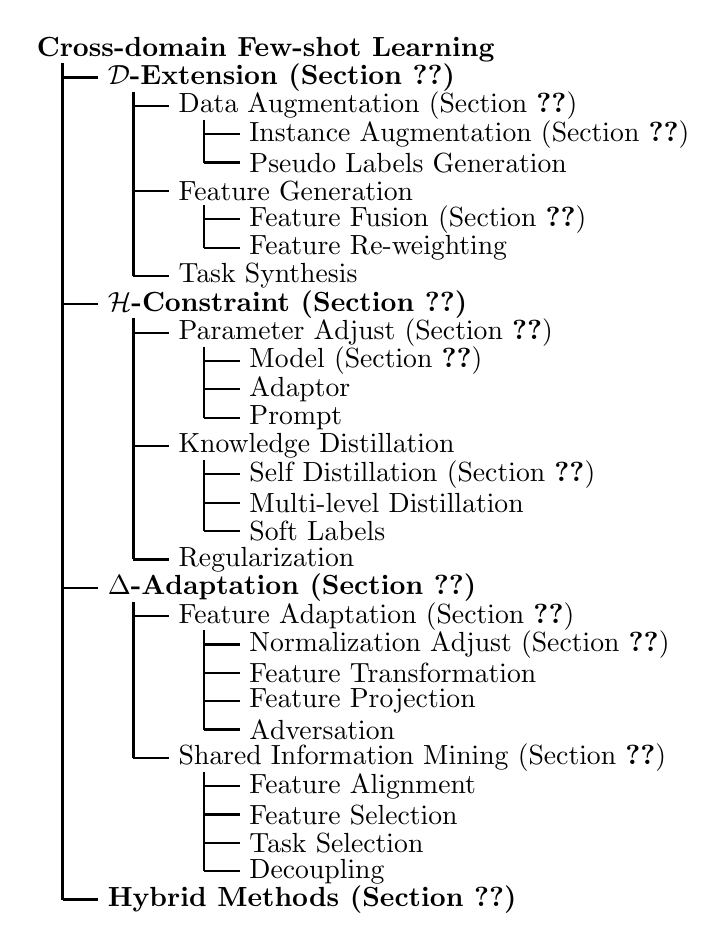
\begin{tikzpicture}[xscale=0.9, yscale=0.36]
\textcolor{black}{
\draw [thick, -] (0, 24) -- (0, 24); \node [right] at (-0.5, 24) {\textbf{Cross-domain Few-shot Learning
}};
\draw [thick, -] (0, 23.5) -- (0, -6);
\draw [thick, -] (0, 23) -- (0.5, 23);\node [right] at (0.5, 23) {\textbf{$\mathcal{D}$-Extension (Section~\ref{instance})}};
\draw [thick, -] (1, 22.5) -- (1, 16);
\draw [thick, -] (1, 22) -- (1.5, 22);\node [right] at (1.5, 22) {Data Augmentation (Section~\ref{sec:FSCIC:dba})};
\draw [thick, -] (2, 21.5) -- (2,20);
\draw [thick, -] (2, 21) -- (2.5, 21);\node [right] at (2.5, 21) {Instance Augmentation (Section~\ref{sec:FSCIC:dba:drbm})};
%\draw [thick, -] (2, 20.5) -- (2,19);
\draw [thick, -] (2, 20) -- (2.5, 20);\node [right] at (2.5, 20) {Pseudo Labels Generation};
\draw [thick, -] (1, 19) -- (1.5, 19);\node [right] at (1.5, 19) {Feature Generation
};
\draw [thick, -] (2, 18.5) -- (2,17);
\draw [thick, -] (2, 18) -- (2.5, 18);\node [right] at (2.5, 18) {Feature Fusion (Section~\ref{sec:FSCIC:dba:drbm})};
%\draw [thick, -] (2, 20.5) -- (2,19);
\draw [thick, -] (2, 17) -- (2.5, 17);\node [right] at (2.5, 17) {Feature Re-weighting};
\draw [thick, -] (1, 16) -- (1.5, 16);\node [right] at (1.5, 16) {Task Synthesis
};
\draw [thick, -] (0, 15) -- (0.5, 15);\node [right] at (0.5, 15) {\textbf{$\mathcal{H}$-Constraint (Section~\ref{hypothesis})}};
\draw [thick, -] (1, 14.5) -- (1, 6);
\draw [thick, -] (1, 14) -- (1.5, 14);\node [right] at (1.5, 14) {Parameter Adjust (Section~\ref{sec:FSCIC:dba})};
\draw [thick, -] (2, 13.5) -- (2,11);
\draw [thick, -] (2, 13) -- (2.5, 13);\node [right] at (2.5, 13) {Model (Section~\ref{sec:FSCIC:dba:drbm})};
%\draw [thick, -] (2, 20.5) -- (2,19);
\draw [thick, -] (2, 12) -- (2.5, 12);\node [right] at (2.5, 12) {Adaptor};
\draw [thick, -] (2, 11) -- (2.5, 11);\node [right] at (2.5, 11) {Prompt};
\draw [thick, -] (1, 10) -- (1.5, 10);\node [right] at (1.5, 10) {Knowledge Distillation
};
\draw [thick, -] (2, 9.5) -- (2,7);
\draw [thick, -] (2,9) -- (2.5, 9);\node [right] at (2.5, 9) {Self Distillation (Section~\ref{sec:FSCIC:dba:drbm})};
%\draw [thick, -] (2, 20.5) -- (2,19);
\draw [thick, -] (2, 8) -- (2.5, 8);\node [right] at (2.5, 8) {Multi-level Distillation};
\draw [thick, -] (2, 7) -- (2.5, 7);\node [right] at (2.5, 7) {Soft Labels};
\draw [thick, -] (1, 6) -- (1.5, 6);\node [right] at (1.5, 6) {Regularization
};
\draw [thick, -] (0, 5) -- (0.5, 5);\node [right] at (0.5, 5) {\textbf{$\Delta$-Adaptation (Section~\ref{adaptation})}};
\draw [thick, -] (1, 4.5) -- (1, -1);
\draw [thick, -] (1, 4) -- (1.5, 4);\node [right] at (1.5, 4) {Feature Adaptation (Section~\ref{sec:FSCIC:dba})};
\draw [thick, -] (2, 3.5) -- (2,0);
\draw [thick, -] (2, 3) -- (2.5, 3);\node [right] at (2.5, 3) {Normalization Adjust (Section~\ref{sec:FSCIC:dba:drbm})};
%\draw [thick, -] (2, 20.5) -- (2,19);
\draw [thick, -] (2, 2) -- (2.5, 2);\node [right] at (2.5, 2) {Feature Transformation};
\draw [thick, -] (2, 1) -- (2.5, 1);\node [right] at (2.5, 1) {Feature Projection};
\draw [thick, -] (2, 0) -- (2.5, 0);\node [right] at (2.5, 0) {Adversation
};
%\draw [thick, -] (2, -0.5) -- (2,-2);
\draw [thick, -] (1,-1) -- (1.5, -1);\node [right] at (1.5, -1) {Shared Information Mining (Section~\ref{sec:FSCIC:dba:drbm})};
\draw [thick, -] (2, -1.5) -- (2,-5);
\draw [thick, -] (2, -2) -- (2.5, -2);\node [right] at (2.5, -2) {Feature Alignment};
\draw [thick, -] (2, -3) -- (2.5, -3);\node [right] at (2.5, -3) {Feature Selection};
\draw [thick, -] (2, -4) -- (2.5, -4);\node [right] at (2.5, -4) {Task Selection};
\draw [thick, -] (2, -5) -- (2.5, -5);\node [right] at (2.5, -5) {Decoupling};
\draw [thick, -] (0, -6) -- (0.5, -6);\node [right] at (0.5, -6) {\textbf{Hybrid Methods (Section~\ref{hybrid})}};}
\end{tikzpicture}}
\vspace{-10pt}
\caption{\textcolor{black}{The taxonomy of representative methods in CDFSL.}}
\label{out}
\end{figure}
%\end{wrapfigure}
\fi